\chapter{Tools and Technologies}

\justify
{\myprojectname} encompasses a wide range of tools and technologies that facilitate the creation, deployment, and maintenance of applications. From integrated development environments (IDEs) for coding to version control systems (VCS) for collaboration, programming languages, frameworks, database management systems (DBMS), cloud platforms, testing tools, API development tools, code editors, project management platforms, security tools, and monitoring/logging solutions.

\section{Tools}
\justify

The following Tools are used for the development of the Application. These tools are used for Development, Debugging and Testing of the Application.


\begin{enumerate}[label=\roman*.]
  \item \textbf{Visual Studio Code}: Visual Studio Code is used to design the OSINT Software, Backend of the Application and Android App Development. Visual Studio Code is a lightweight Code Editor for the development of the different kinds of Applications and Softwares. It is developed by Microsoft Inc. for developers developing for Windows, Linux, MacOS and Android. \cite{VSCode}
  
  \item \textbf{Flipper}: The Flipper is used for debugging the Android Application. It provides different debugging plugins such as logcat, Image Compressing, Shared Preferences, Network logs and SQLite Database visualization. The Flipper is developed by Facebook. \cite{FLP}
  
  \item \textbf{React Native Debugger}:  React Native debugger is used for debugging components rendering on different screens and their structure, alignment and styling. \cite{RDT}
  
  \item \textbf{HTTPie}:   HTTPie is used for testing of the APIs of CallOne Application. \cite{Httpie}
  
  \item \textbf{Android Studio}: Android Studio is used for creating Native React Modules in Kotlin. Android Studio is Official Integrated Development Environment for developing Android Applications. \cite{Android Studio}
  
  \item \textbf{Android Emulator}: The Android Emulator simulates Android devices on computer to test application on a variety of devices and Android API levels without needing to have each physical device. \cite{Android Studio}
  
  \item \textbf{Git}: Git is a free and open source distributed version control system designed to handle everything from small to very large projects with speed and efficiency. \cite{Git}
  
  \item \textbf{Chromium Browser}: Chromium is an open-source browser project that aims to build a safer, faster, and more stable way for all users to experience the web. \cite{Chromium}

  \item \textbf{DBeaver}: DBeaver is cross-platform database tool for developers, database administrators, analysts, and everyone working with data. It supports all popular SQL databases like MySQL, MariaDB, PostgreSQL, SQLite, Apache Family, and more. \cite{DBeaver}

  \item \textbf{Nginx}: NGINX accelerates content and application delivery, improves security, and facilitates availability and scalability for the busiest websites. \cite{Nginx}

  \item \textbf{Puppeteer}: Puppeteer is a Node.js library which provides a high-level API to control Chrome/Chromium over the DevTools Protocol. \cite{Puppeteer}
  
\end{enumerate}


\section{Technologies}
\justify

The following Technologies are used for the development of the Application.

\begin{enumerate}[label=\roman*.]
  \item \textbf{React Native}: React Native is JavaScript based Native Application Development Framework. It allows to build natively-rendered mobile Applications for Android and iOS. \cite{RN}
  
  \item \textbf{Kotlin}: Kotlin is a programming language used for development of Android Applications. \cite{kt}
  
  \item \textbf{TypeScript}: TypeScript adds additional syntax to JavaScript to support a tighter integration with code editor. It Catch errors early in code editor. \cite{TypeScript}
  
  \item \textbf{Express.js}: Express is a minimal and flexible Node.js web application framework that provides a robust set of features for web and mobile applications. \cite{Express}
  
  \item \textbf{Node.js}: Node.js is a free, open-source, cross-platform JavaScript runtime environment that lets developers create servers, web apps, command line tools and scripts. It is built on Chrome's Javascript V8 engine. \cite{Node}
  
  \item \textbf{Crypto-js}: Crypto-js is javaScript implementations of standard and secure cryptographic algorithms. CryptoJS is a growing collection of standard and secure cryptographic algorithms implemented in JavaScript using best practices and patterns. \cite{Crypto-js}

  \item \textbf{PostgreSQL}: PostgreSQL is a powerful open-source relational database management system known for its reliability, robustness, and extensibility. It offers a wide range of advanced features, including support for complex queries, indexing, and transactions. \cite{psql}
 
  \item \textbf{React Native Firebase}: React Native Firebase is the officially recommended collection of packages that brings React Native support for all Firebase services on both Android and iOS apps. \cite{RNF}
  
  \item \textbf{JSON Web Tokens (JWT)}: JSON Web Tokens are an open, industry standard RFC 7519 method for representing claims securely between two parties. \cite{JWT}
  
  \item \textbf{PDFKit}: PDFKit is a PDF document generation library for Node and the browser that makes creating complex, multi-page, printable documents easy. \cite{PDFKit}
  
  \item \textbf{Baileys (WhatsApp Client)}: Baileys is a Whatsapp client to communicate with web sockets. \cite{Baileys}
  

  % \begin{figure}
  %   \centering
  %   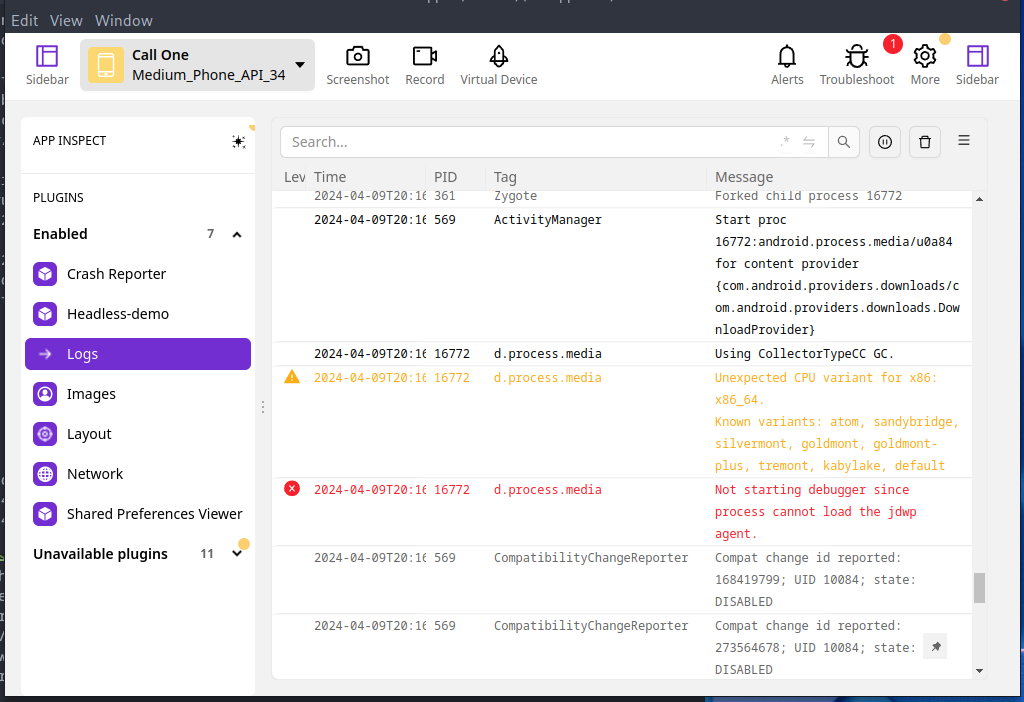
\includegraphics[width=1\linewidth]{Media//Chapter 6/flipper.png}
  %   \caption{Flipper Debugging}
  %   \label{fig:Flipper Debugging Tool}
  % \end{figure}
\end{enumerate}